\chapter{Autoencoders}

Traditional supervised learning requires labeled data. Autoencoders were created to answer a fundamental question: \emph{Can a neural network learn useful features from unlabeled data?} This is called \textbf{representation learning}.

A \textbf{representation} (embedding / latent vector) is a compact vector that captures the important information in the input. 
\[
\text{Example: Image } (150,528 \text{ pixels}) \longrightarrow \text{Embedding } (128 \text{ numbers})
\]

The goal is not just compression, but \textbf{preserving meaningful information}. Once a good embedding is learned, it can be reused for many downstream tasks: Classification, Object Detection, Segmentation, and more. This core idea is heavily utilized in modern foundation models such as BERT, GPT, and CLIP. Autoencoders were among the first neural networks designed specifically for learning embeddings.

\section*{Why Not PCA?}
Principal Component Analysis (PCA) also reduces dimensionality, but it has important limitations:
\begin{itemize}
    \item Works only with \textbf{linear relationships}.
    \item Cannot learn hierarchical features ($\text{edge} \rightarrow \text{eyes} \rightarrow \text{faces}$).
    \item Has a fixed linear transformation after training.
\end{itemize}
Autoencoders use deep neural networks, allowing them to learn complex non-linear representations.

\section{Vanilla Autoencoders}

\subsection{The Big Idea}
Autoencoders were introduced to solve the problem of learning useful representations without labels. Instead of predicting classes, they learn by reconstructing their own inputs. An encoder compresses the input into a low-dimensional latent representation, and a decoder reconstructs the original data from that representation. The bottleneck prevents the network from simply copying the input, forcing it to retain only the most informative features.

This simple reconstruction principle laid the foundation for many modern models including VAE, VQ-VAE, MAE, and the latent encoders used in Stable Diffusion.

Researchers proposed an elegant principle: instead of training a network with explicit supervision (\emph{``classify this image''}), instruct it to \emph{``compress this image, then reconstruct it''}. If the reconstruction is accurate, the compressed vector must preserve essential semantic information. In other words, the network learns representations without human labels.

\[
\text{Original Image} \longrightarrow \text{Encoder} \longrightarrow \text{Latent Vector} \longrightarrow \text{Decoder} \longrightarrow \text{Reconstructed Image}
\]

The training objective is:
\[
\text{Reconstructed Image} \approx \text{Original Image}
\]
No human labels are required because the image supervises itself. This makes autoencoders one of the earliest and purest forms of \textbf{self-supervised learning}.

\subsection{The Bottleneck}
The latent vector is intentionally constrained to be much smaller than the input:
\[
\text{Input } (150,528 \text{ values}) \longrightarrow \text{Bottleneck } (128 \text{ values}) \longrightarrow \text{Output } (150,528 \text{ values})
\]
This \textbf{bottleneck} forces the model to retain only the most critical information instead of trivially memorizing every pixel.

\subsection{Architecture of a Vanilla Autoencoder}


A vanilla autoencoder consists of two main component networks:
\begin{enumerate}
    \item \textbf{Encoder}: Compresses the high-dimensional input into a low-dimensional latent vector.
    \[
    150,528 \longrightarrow 4096 \longrightarrow 1024 \longrightarrow 256 \longrightarrow 64
    \]
    The final 64-dimensional output is called the \emph{Latent Vector}, \emph{Latent Representation}, or \emph{Embedding}.
    
    \item \textbf{Bottleneck}: Is the narrowest layer of the network where the latent vector is stored. Because information capacity is strictly limited, the network discards fine noise and retains fundamental structural features.
    
    \item \textbf{Decoder}: Reconstructs the original input from the latent vector.
    \[
    64 \longrightarrow 256 \longrightarrow 1024 \longrightarrow 4096 \longrightarrow 150,528
    \]
\end{enumerate}
\clearpage
\begin{figure}[htbp]
    \centering
    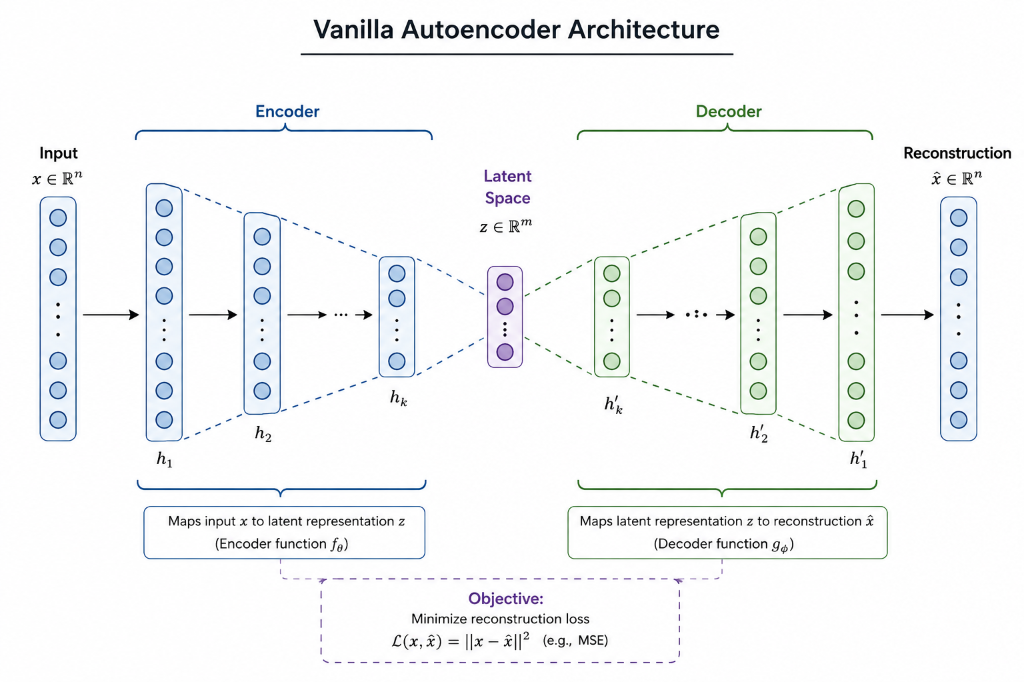
\includegraphics[width=0.85\linewidth]{figures/fig_8_vanilla_autoencoder_architecture.png}
    \caption{Vanilla Autoencoder Architecture showing Encoder, Latent Space, and Decoder.}
    \label{fig:vanilla_autoencoder_architecture}
\end{figure} 

\subsection{Training \& Reconstruction Loss}



During training, the reconstructed image $\hat{x}$ is compared with the original input $x$ using a \textbf{Reconstruction Loss}. For images, the most common loss function is Mean Squared Error (MSE):
\[
\mathcal{L}_{\text{recon}} = \| x - \hat{x} \|^2
\]
Backpropagation updates parameters across both the encoder and decoder simultaneously. Because the bottleneck restricts throughput, the encoder is forced to learn meaningful representations rather than simple copying.
\clearpage
\begin{figure}[htbp]
    \centering
    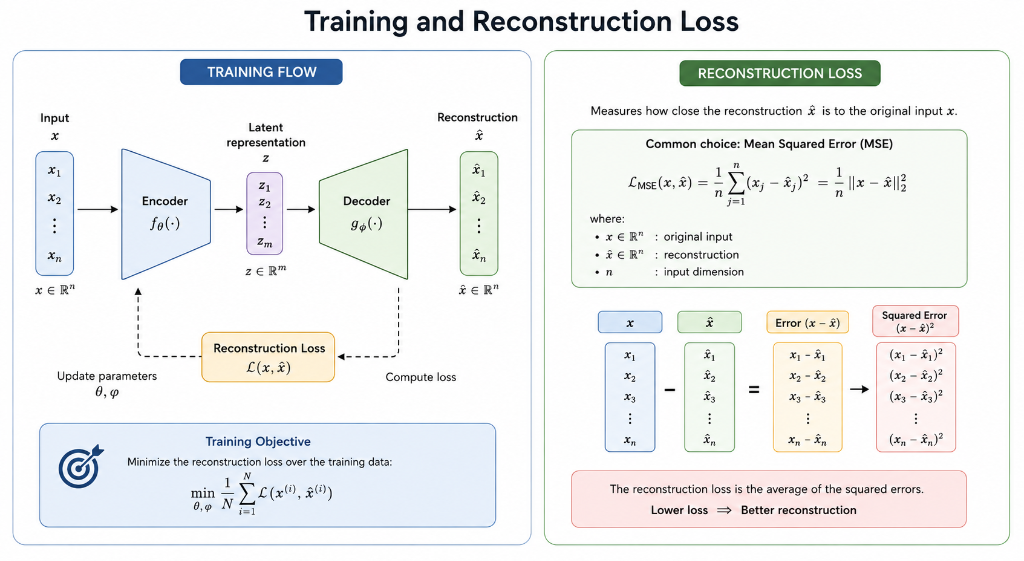
\includegraphics[width=0.95\linewidth]{figures/fig_8_training_and_reconstruction_loss.png}
    \caption{Training Flow and Reconstruction Loss formulation, showing Mean Squared Error (MSE) calculation across pixel dimensions and gradient update loops.}
    \label{fig:training_and_reconstruction_loss}
\end{figure}

\subsection*{Summary}
A vanilla autoencoder is composed of an encoder, a latent representation (bottleneck), and a decoder. The encoder compresses the input into a compact embedding, while the decoder reconstructs the original input from that embedding. During training, the reconstructed image is compared with the original using a reconstruction loss, and backpropagation updates both networks. Because the bottleneck severely limits the amount of information that can pass through, the encoder is forced to learn meaningful representations instead of simply copying the input.

\section{Latent Space Properties}

A \textbf{latent space} is the mathematical space containing all latent vectors (embeddings) produced by the encoder:
\begin{itemize}
    \item 2-dimensional latent vector $\longrightarrow$ 2D latent space
    \item 64-dimensional latent vector $\longrightarrow$ 64D latent space
\end{itemize}

Every input image becomes a point in this space where \textbf{similar inputs lie close together}. Without explicit labels, the encoder naturally clusters similar images because they require similar feature representations for accurate reconstruction. The latent space organizes data by \textbf{semantic similarity}, not raw pixel values. This property is crucial for:
\begin{itemize}
    \item Image Retrieval
    \item Clustering
    \item Similarity Search
\end{itemize}

\begin{figure}[htbp]
    \centering
    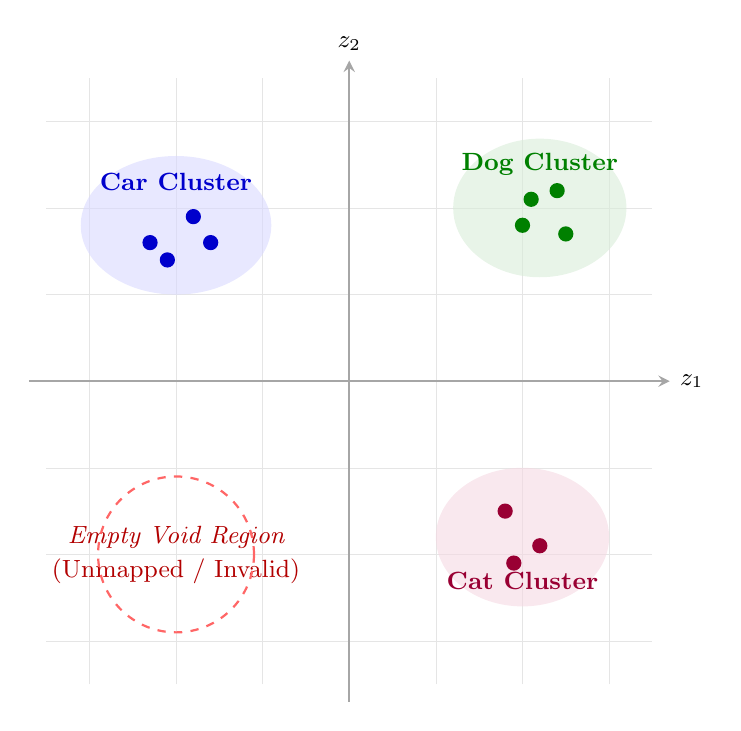
\begin{tikzpicture}[scale=1.1, >=stealth]
        % Background grid & axes
        \draw[very thin, color=gray!20] (-3.5,-3.5) grid (3.5,3.5);
        \draw[->, thick, color=gray!70] (-3.7,0) -- (3.7,0) node[right, black] {\small $z_1$};
        \draw[->, thick, color=gray!70] (0,-3.7) -- (0,3.7) node[above, black] {\small $z_2$};

        % Car Cluster (Top Left)
        \fill[blue!15, opacity=0.6] (-2,1.8) ellipse (1.1cm and 0.8cm);
        \node[blue!80!black, font=\bfseries\small] at (-2,2.3) {Car Cluster};
        \fill[blue!80!black] (-2.3,1.6) circle (2.5pt);
        \fill[blue!80!black] (-1.8,1.9) circle (2.5pt);
        \fill[blue!80!black] (-2.1,1.4) circle (2.5pt);
        \fill[blue!80!black] (-1.6,1.6) circle (2.5pt);

        % Dog Cluster (Top Right)
        \fill[green!50!black!15, opacity=0.6] (2.2,2.0) ellipse (1.0cm and 0.8cm);
        \node[green!50!black, font=\bfseries\small] at (2.2,2.5) {Dog Cluster};
        \fill[green!50!black] (2.0,1.8) circle (2.5pt);
        \fill[green!50!black] (2.4,2.2) circle (2.5pt);
        \fill[green!50!black] (2.1,2.1) circle (2.5pt);
        \fill[green!50!black] (2.5,1.7) circle (2.5pt);

        % Cat Cluster (Bottom Right)
        \fill[purple!15, opacity=0.6] (2.0,-1.8) ellipse (1.0cm and 0.8cm);
        \node[purple!80!black, font=\bfseries\small] at (2.0,-2.3) {Cat Cluster};
        \fill[purple!80!black] (1.8,-1.5) circle (2.5pt);
        \fill[purple!80!black] (2.2,-1.9) circle (2.5pt);
        \fill[purple!80!black] (1.9,-2.1) circle (2.5pt);

        % Empty Void Region (Bottom Left)
        \node[red!70!black, font=\itshape\small] at (-2.0,-1.8) {Empty Void Region};
        \node[red!70!black, font=\small] at (-2.0,-2.2) {(Unmapped / Invalid)};
        \draw[red!60, dashed, thick] (-2.0,-2.0) circle (0.9cm);
    \end{tikzpicture}
    \caption{Visualization of a 2D Latent Space learned by an Autoencoder. Similar semantic concepts (Cars, Dogs, Cats) naturally form clustered regions, while unpopulated areas represent empty void regions.}
    \label{fig:latent_space_visualization}
\end{figure}

\subsection{Latent Interpolation}
Suppose we take two latent vectors corresponding to a \textbf{DOG} at $(2, 3)$ and a \textbf{WOLF} at $(8, 5)$. What happens if we step gradually between them in the latent space?
\begin{align*}
(2, 3.0) &\longrightarrow \text{DOG} \\
(3, 3.5) &\longrightarrow \text{Dog-like} \\
(4, 4.0) &\longrightarrow \text{Half Dog, Half Wolf} \\
(5, 4.5) &\longrightarrow \text{Wolf-like} \\
(8, 5.0) &\longrightarrow \text{WOLF}
\end{align*}
Moving smoothly between latent vectors generates smooth transitions upon decoding. The decoder synthesizes intermediate images that were never in the original dataset. This operation is called \textbf{latent interpolation}.

\subsection{Limitation of Vanilla Autoencoders}
Because a vanilla autoencoder only maps training inputs to deterministic points, large portions of the latent space remain completely unmapped (empty regions).
\clearpage
\begin{figure}[htbp]
    \centering
    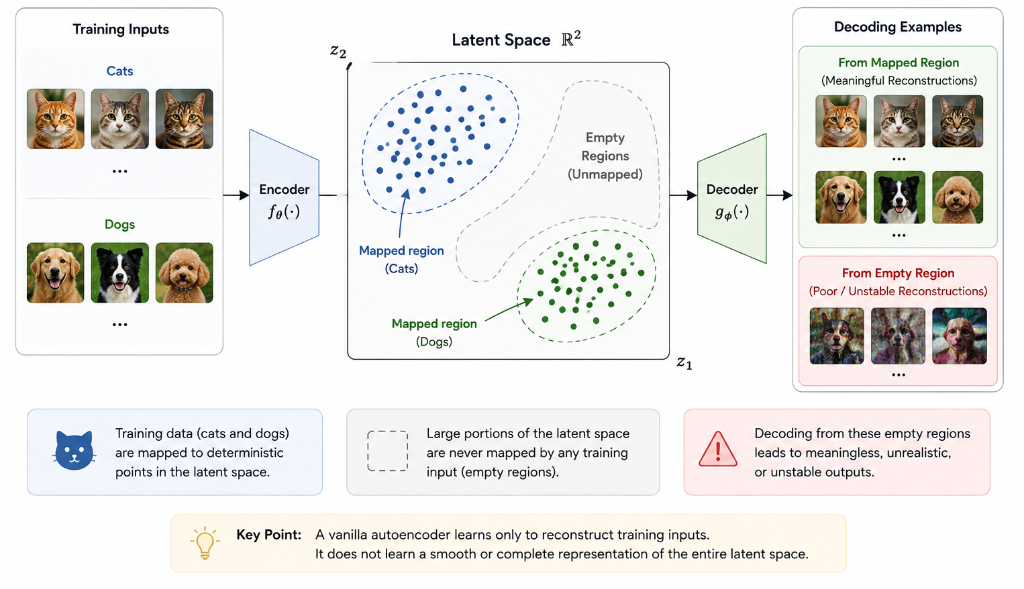
\includegraphics[width=0.95\linewidth]{figures/fig_8_latent_space_empty_regions.png}
    \caption{Deterministic latent space mapping in a Vanilla Autoencoder. Training data (Cats and Dogs) are mapped to isolated regions, leaving large unmapped empty regions where decoding yields poor or unstable reconstructions.}
    \label{fig:latent_space_empty_regions}
\end{figure}

\begin{itemize}
    \item If a random vector $\mathbf{z}$ is sampled from an empty region, the decoder outputs blurry or non-sensical artifacts because it was never trained on that area.
    \item Interpolation works well between nearby points ($\text{Dog} \rightarrow \text{Wolf}$), but fails across distant points ($\text{Dog} \rightarrow \text{Airplane}$) when the straight-line trajectory crosses unmapped empty space.
\end{itemize}
Thus, classical autoencoders are \textbf{poor generative models}. This fundamental limitation directly motivates the development of \textbf{Variational Autoencoders (VAEs)}.

\subsection*{Summary}
A latent space is the space formed by all latent vectors produced by the encoder. Each input is mapped to a point in the space, and similar inputs naturally tend to lie close together because they require similar representations for reconstruction. Distances in the latent space therefore reflect semantic similarity rather than raw pixel similarity, making operations such as clustering, retrieval, and interpolation possible. However, classical autoencoders produce latent spaces with large empty regions, making random sampling unreliable. This fundamental limitation motivates Variational Autoencoders (VAEs), which are designed to learn a smooth, continuous latent space suitable for generation.

\subsection*{Why Vanilla Autoencoders Fail?}
A vanilla autoencoder maps each training image to a latent vector; only these points are learned, and most of the latent space is empty. If we sample a random latent vector and decode it, the decoder often produces blurry or meaningless outputs because it has never seen that region during training. During training, the decoder only receives latent vectors produced by the encoder—it never learns how to decode arbitrary random vectors.

The latent space consists of isolated points or clusters separated by empty regions; there is no guarantee that points in the empty regions correspond to valid images:
\begin{itemize}
    \item Interpolation works well when two latent vectors are close (e.g., $\text{Dog} \rightarrow \text{Wolf}$).
    \item Interpolation may fail when they are far apart (e.g., $\text{Dog} \rightarrow \text{Airplane}$) because the path crosses empty regions.
\end{itemize}

A vanilla autoencoder is deterministic: for one input, it produces the exact same latent vector every time. There is:
\begin{itemize}
    \item No uncertainty
    \item No probability distribution
    \item No variability
\end{itemize}
Instead of isolated points, we want continuous regions in the latent space so that any point inside the region decodes to a valid image.

\section{Variational Autoencoders (VAE)}

To fix the empty region problem, a \textbf{Variational Autoencoder (VAE)} replaces single deterministic latent points with \textbf{continuous probability distributions}.

\begin{figure}[htbp]
    \centering
    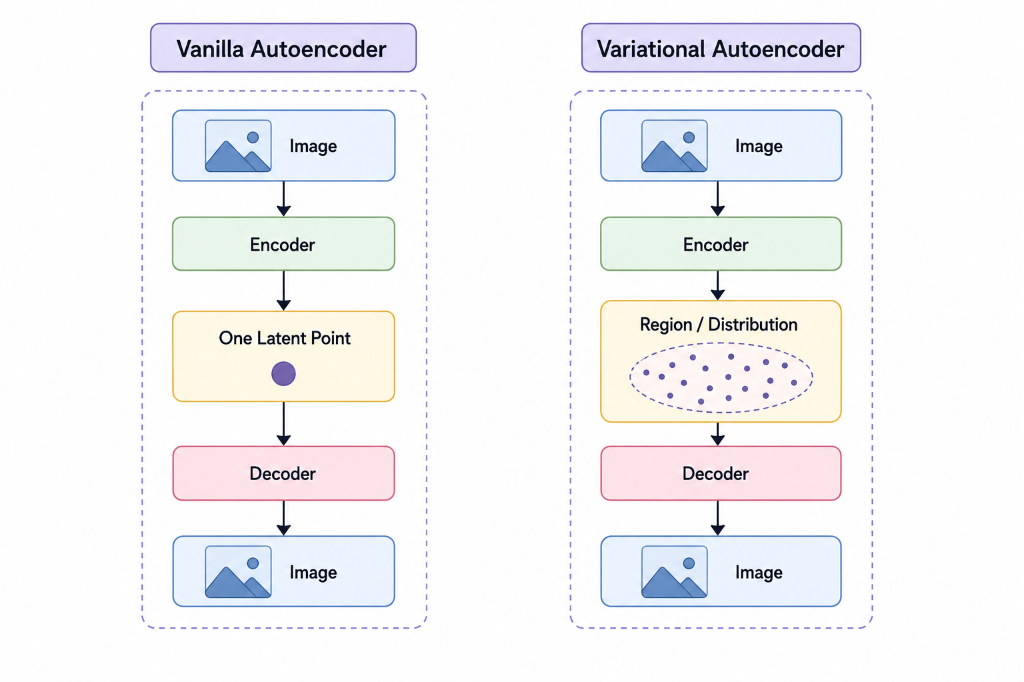
\includegraphics[width=0.85\linewidth]{figures/fig_8_vanilla_vs_vae.png}
    \caption{Comparison between Vanilla Autoencoders (mapping inputs to single isolated latent points) and Variational Autoencoders (mapping inputs to continuous probability distributions).}
    \label{fig:vanilla_vs_vae}
\end{figure}

\subsection{Why Probability Distributions?}
Consider representing a dog: every dog should not map to a single isolated point because dogs vary in color, size, posture, and breed, yet all belong to the concept of a dog. Instead of stating \emph{``this dog is exactly at point $(x,y)$''}, a VAE specifies \emph{``this dog belongs to a region centered around $\boldsymbol{\mu}$ with spread $\boldsymbol{\sigma}^2$''}.

A Gaussian latent region is fully defined by two parameter vectors produced by the encoder:
\begin{itemize}
    \item \textbf{Mean Vector ($\boldsymbol{\mu}$)}: The center of the region (most likely representation).
    \item \textbf{Log Variance Vector ($\log \boldsymbol{\sigma}^2$)}: The extent or radius of allowable variation.
\end{itemize}

\begin{figure}[htbp]
    \centering
    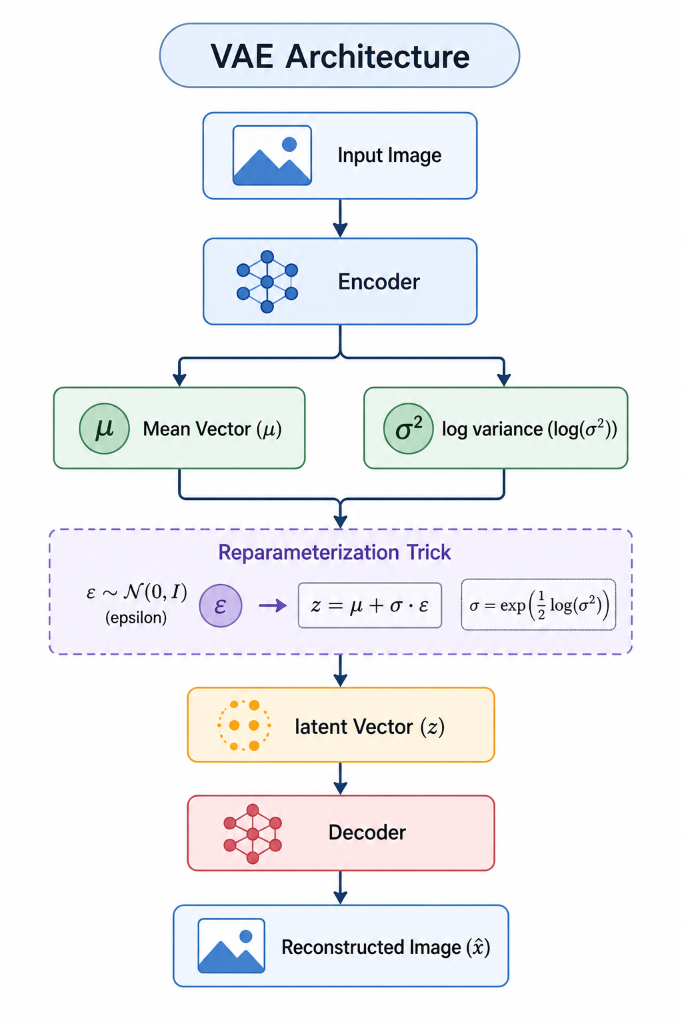
\includegraphics[width=0.85\linewidth]{figures/fig_8_vae_architecture.png}
    \caption{Detailed VAE Architecture incorporating the Reparameterization Trick to enable end-to-end backpropagation.}
    \label{fig:vae_architecture}
\end{figure}

\subsection{The Reparameterization Trick}

\subsubsection*{Why We Sample the Latent Vector}
We sample the latent vector $\mathbf{z}$ because we want the decoder to learn that an image is represented by an entire continuous region in the latent space rather than by a single fixed point. If we always used the mean vector $\boldsymbol{\mu}$ directly, every input would consistently produce the exact same latent representation, causing the model to behave similarly to a classical deterministic autoencoder.

By sampling different latent vectors $\mathbf{z}$ from the Gaussian distribution defined by $\boldsymbol{\mu}$ and $\boldsymbol{\sigma}^2$, the decoder learns to reconstruct valid images from many nearby points. This creates a smooth, continuous latent space where small changes in $\mathbf{z}$ lead to small changes in the generated image, enabling the VAE to generate novel and diverse samples.

\subsubsection*{Mathematical Formulation \& Gradient Flow}
However, directly sampling $\mathbf{z} \sim \mathcal{N}(\boldsymbol{\mu}, \boldsymbol{\sigma}^2)$ is a random operation, and random operations are non-differentiable, which blocks backpropagation. 

To solve this, VAE introduces the \textbf{Reparameterization Trick}. Instead of sampling $\mathbf{z}$ directly, we first sample independent standard Gaussian noise $\boldsymbol{\epsilon} \sim \mathcal{N}(0, \mathbf{I})$ and then compute the latent vector deterministically:
\[
\mathbf{z} = \boldsymbol{\mu} + \boldsymbol{\sigma} \odot \boldsymbol{\epsilon}
\]
This moves the randomness into $\boldsymbol{\epsilon}$, which is independent of the network, while $\boldsymbol{\mu}$ and $\boldsymbol{\sigma}$ remain differentiable outputs of the encoder. As a result, gradients flow through the encoder during backpropagation, allowing the entire VAE to be trained end-to-end.

\subsubsection*{Step-by-Step Execution Example}
Consider a concrete step-by-step example of passing a dog image through the VAE:
\begin{enumerate}
    \item \textbf{Encoder Prediction}: We feed the dog image into the encoder. Unlike a vanilla autoencoder, the encoder does not output one latent vector; instead, it outputs two parameter vectors:
    \[
    \boldsymbol{\mu} = [2.3, 1.8], \quad \boldsymbol{\sigma}^2 = [0.1, 0.2]
    \]
    The encoder indicates: \emph{``I think this dog belongs around here in the latent space, but I am not going to pick one exact point.''} Thus, we have a continuous region instead of a single isolated point.

    \item \textbf{Sampling $\mathbf{z}$ via Noise}: We need one latent vector to send to the decoder, but we do not use $\boldsymbol{\mu}$ directly. Instead, we first generate random noise from a standard Gaussian distribution, e.g., $\boldsymbol{\epsilon} = [0.4, -0.8] \sim \mathcal{N}(0, \mathbf{I})$. We then combine it with $\boldsymbol{\mu}$ and $\boldsymbol{\sigma}$ using $z = \boldsymbol{\mu} + \boldsymbol{\sigma} \odot \boldsymbol{\epsilon}$ to form the latent vector $\mathbf{z}$.

    \item \textbf{Decoder Reconstruction}: The decoder receives $\mathbf{z}$ and reconstructs the original dog image. Now, if we later pick a new point inside the region that the decoder has never seen before, it can still generate a realistic dog image.
\end{enumerate}

\section{Vector Quantized VAE (VQ-VAE)}

A \textbf{VQ-VAE} (Vector Quantized Variational Autoencoder, Van den Oord et al., 2017) replaces the continuous Gaussian latent space of a standard VAE with a \textbf{discrete Codebook}. The encoder still produces a continuous latent vector $z_e$, but it is immediately quantized by replacing it with the nearest codebook entry $z_q$. The decoder then reconstructs the image from this discrete representation.

This allows images to be represented as sequences of reusable \textbf{visual tokens} instead of arbitrary floating-point vectors, making VQ-VAE a foundational architecture for token-based generative models such as the original DALL-E and VQGAN.

\subsection*{Motivation: Continuous vs. Discrete Latent Spaces}
In a standard VAE, every image—even nearly identical images—maps to slightly different continuous latent points. For instance, subtle variations of a blue color might yield continuous vectors like:
\[
(124, 201, 87), \quad (124, 202, 88), \quad (125, 201, 86), \dots
\]
resulting in millions of redundant continuous possibilities.

The main idea of VQ-VAE is that instead of allowing arbitrary latent vectors, the encoder is forced to choose from a fixed, learned dictionary called a \textbf{Codebook}:
\begin{figure}[htbp]
    \centering
    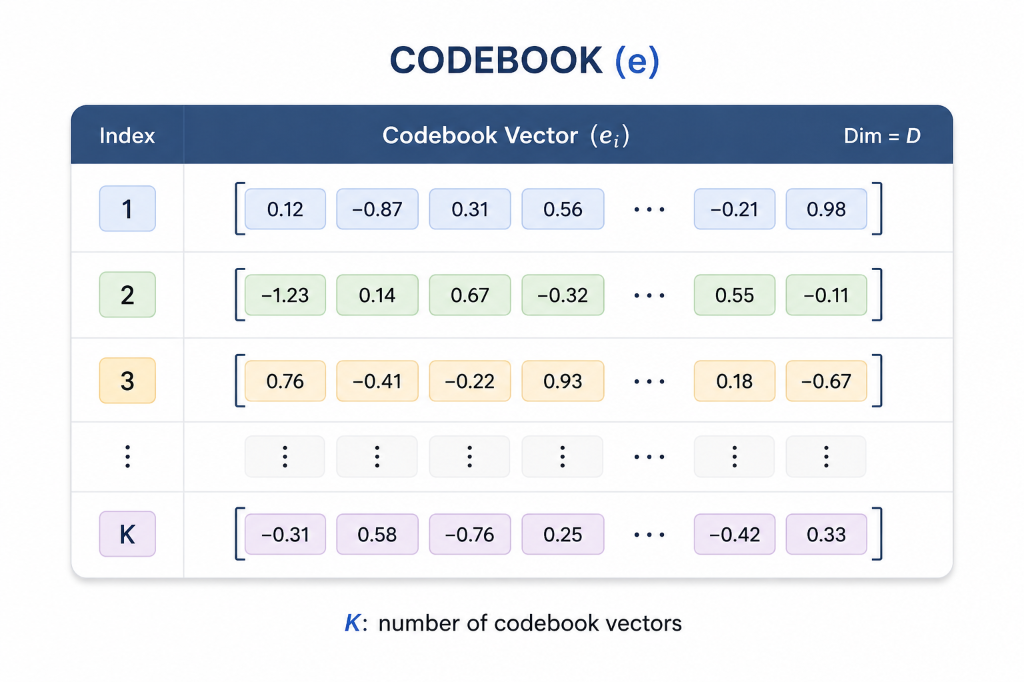
\includegraphics[width=0.85\linewidth]{figures/fig_8_codebook_table.png}
    \caption{Structure of the discrete Codebook $\mathcal{E}$ containing $K$ feature vectors of dimension $D$.}
    \label{fig:codebook_table}
\end{figure}

\begin{minipage}[t]{0.45\textwidth}
\begin{itemize}
    \item \textbf{Entry 1}: Round eye feature
    \item \textbf{Entry 2}: Green grass texture
    \item \textbf{Entry 3}: Blue sky
    \item \textbf{Entry 4}: Curved brown edge
\end{itemize}
\end{minipage}
\hfill
\begin{minipage}[t]{0.50\textwidth}
\vspace{0.3cm} % Move the text down
These semantic entry representations are not manually engineered; instead, they are discovered automatically by the model during end-to-end training.
\end{minipage}

\begin{figure}[htbp]
	\centering
	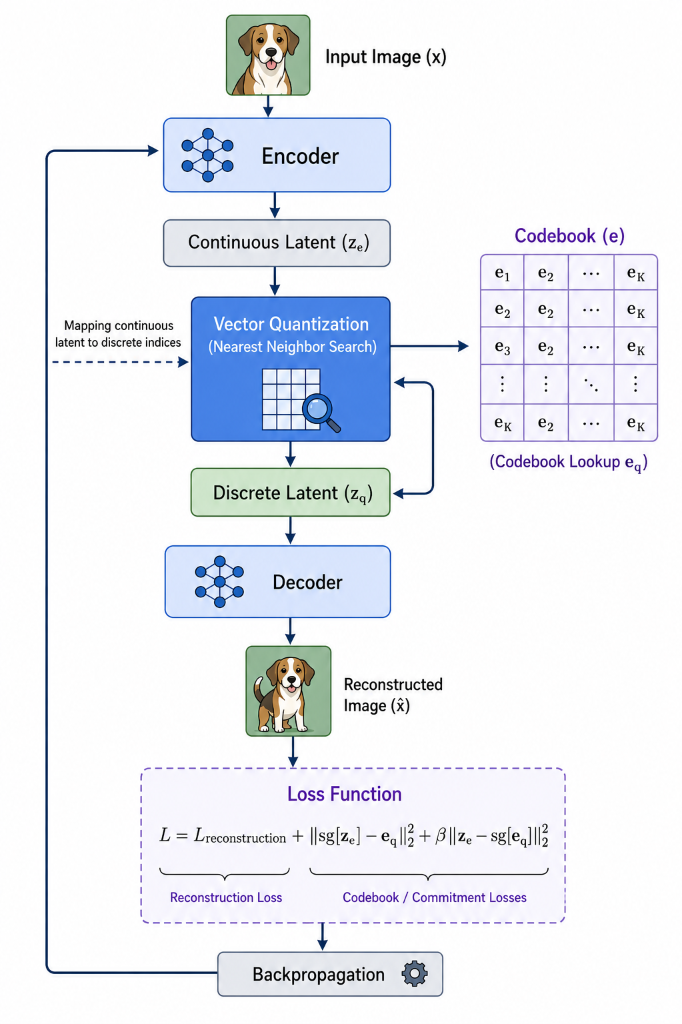
\includegraphics[width=0.85\linewidth]{figures/fig_8_vqvae_architecture.png}
	\caption{VQ-VAE Architecture showing Vector Quantization over a discrete codebook dictionary and loss formulation.}
	\label{fig:vqvae_architecture}
\end{figure}
\clearpage
\subsection{Vector Quantization Mechanism}
Instead of generating a single vector for an entire image, the encoder extracts spatial features and outputs a continuous latent vector $z_e(x)$ for each image patch. For each patch vector, the quantization layer searches the codebook dictionary $\mathcal{E} = \{e_1, e_2, \dots, e_K\}$ for the nearest vector entry in Euclidean distance:
\[
z_q(x) = e_k, \quad \text{where } k = \arg\min_j \| z_e(x) - e_j \|_2
\]



\subsubsection*{Example: From Image Patches to Discrete Visual Tokens}

Consider a dog image processed by a VQ-VAE. The quantization process converts each continuous latent feature into its nearest codebook entry.

\paragraph{Step 1. Continuous Latent Features}

After encoding, each spatial patch is represented by a continuous feature vector:

\[
\begin{array}{ccl}
\textbf{Patch 1} &:& (2.4,\;1.6)\;\rightarrow\;\text{Codebook Entry }81\\
\textbf{Patch 2} &:& (-1.1,\;0.8)\;\rightarrow\;\text{Codebook Entry }205\\
\textbf{Patch 3} &:& (0.5,\;1.2)\;\rightarrow\;\text{Codebook Entry }511\\
&\vdots&\\
\textbf{Patch N} &:& (1.7,\;0.1)\;\rightarrow\;\text{Codebook Entry }98
\end{array}
\]

Each continuous vector is replaced by the nearest prototype stored in the learned codebook.

\vspace{0.4cm}

\paragraph{Step 2. Image as a Sequence of Visual Tokens}

Instead of storing floating-point vectors, the image is represented only by the selected codebook indices:

\[
\boxed{
[81,\;205,\;511,\;\ldots,\;98]
}
\]

These indices are called \textbf{visual tokens}. Similar to how a sentence is represented by a sequence of words, an image can be represented by a sequence of discrete codebook entries.

\vspace{0.4cm}

\paragraph{Step 3. Quantization and Reconstruction}

Assume the encoder outputs

\[
z_e=[2.4,\;1.6].
\]

The nearest codebook vector is

\[
e_2=[2.6,\;1.5].
\]

The quantization layer performs

\[
z_q=e_2=[2.6,\;1.5].
\]

The original continuous representation is discarded, and only the quantized vector is forwarded to the decoder.

\vspace{0.3cm}

\begin{center}
\fbox{
\parbox{0.92\linewidth}{
\textbf{Key Idea}

The decoder never receives the encoder output $z_e$ directly. Instead, it reconstructs the image exclusively from the quantized representation $z_q$, ensuring that every latent feature belongs to the finite codebook.
}
}
\end{center}

\subsection{Loss Function \& Training Objective}
Because the $\arg\min$ operation in vector quantization is non-differentiable, straight-through gradient estimators are used. The total training objective combines reconstruction loss with codebook optimization and commitment penalties:
\[
\mathcal{L} = \mathcal{L}_{\text{reconstruction}} + \|\text{sg}[z_e] - e_q\|_2^2 + \beta \|z_e - \text{sg}[e_q]\|_2^2
\]
where $\text{sg}[\cdot]$ denotes the stop-gradient operator.
\begin{itemize}
    \item \textbf{Reconstruction Loss}: $\mathcal{L}_{\text{reconstruction}} = \|x - \hat{x}\|^2$ penalizes reconstruction errors.
    \item \textbf{Codebook Loss}: $\|\text{sg}[z_e] - e_q\|_2^2$ moves dictionary codebook vectors toward encoder outputs.
    \item \textbf{Commitment Loss}: $\beta \|z_e - \text{sg}[e_q]\|_2^2$ prevents encoder outputs from fluctuating wildly between dictionary entries.
\end{itemize}

\subsection*{Summary Comparison: VAE vs. VQ-VAE}
\begin{itemize}
    \item \textbf{Variational Autoencoder (VAE)}: The latent representation is \textbf{continuous} and obtained by sampling from a Gaussian probability distribution $\mathcal{N}(\boldsymbol{\mu}, \boldsymbol{\sigma}^2)$.
    \item \textbf{Vector Quantized VAE (VQ-VAE)}: The latent representation is \textbf{discrete} and obtained by selecting the nearest vector entry from a learned codebook dictionary.
\end{itemize}

\section{Denoising Autoencoders (DAE)}

In a vanilla autoencoder, the input and the target are identical. Researchers realized something critical: \emph{``The network might simply learn to copy the image.''} Even with a bottleneck, the model sometimes focuses on reconstructing low-level pixel details instead of learning robust features.

\subsection*{The Core Idea}
Instead of feeding the original clean image $x$, we feed a corrupted, noisy image $\bar{x}$:
\[
\bar{x} = x + \text{noise}
\]
\clearpage
\begin{figure}[htbp]
    \centering
    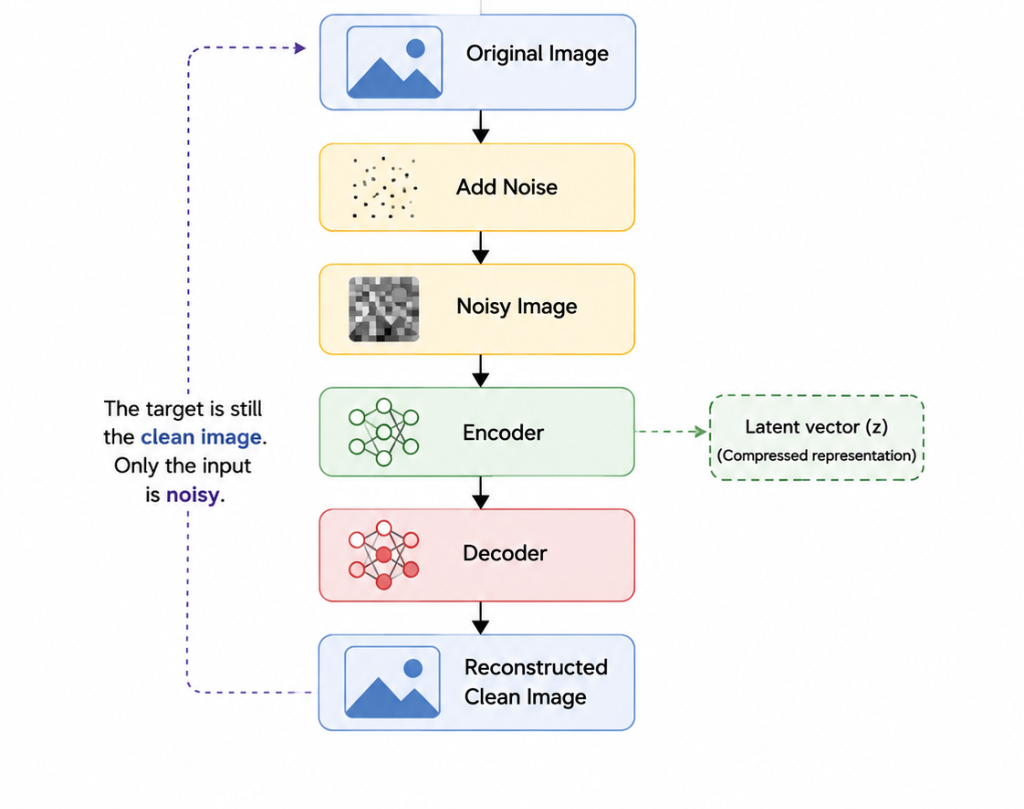
\includegraphics[width=0.85\linewidth]{figures/fig_8_denoising_autoencoder.png}
    \caption{Denoising Autoencoder pipeline: adding noise to clean inputs ($\bar{x} = x + \text{noise}$) and training the network to reconstruct the original clean target ($x$).}
    \label{fig:denoising_autoencoder}
\end{figure}



Mean Squared Error (MSE) loss and backpropagation are used to train the network. \textbf{Crucially, the target is still the clean image $x$; only the input is noisy ($\bar{x}$).}

\subsection*{Learning Robust Features}
Instead of memorizing raw pixels, the model learns meaningful representations:
\begin{itemize}
    \item Edges
    \item Shapes
    \item Textures
    \item Object structure
\end{itemize}
These learned features are significantly more useful for downstream tasks.

\subsection*{Connection to Diffusion Models}
Many modern generative architectures are based on exactly this denoising concept. The prominent example is \textbf{Diffusion Models}, which execute denoising via either of two equivalent targets:
\begin{center}
\begin{tabular}{ccc}
\fbox{\parbox{0.38\linewidth}{\centering \textbf{Noisy Image } ($\bar{x}$)\\[2pt]$\downarrow$\\[2pt]\textbf{Predict Clean Image } ($x$)}} & \quad $\mathbf{OR}$ \quad & \fbox{\parbox{0.38\linewidth}{\centering \textbf{Noisy Image } ($\bar{x}$)\\[2pt]$\downarrow$\\[2pt]\textbf{Predict Noise } ($\epsilon$)}}
\end{tabular}
\end{center}

\section{Sparse Autoencoders (SAE)}

If we have a latent vector containing 512 neurons, a vanilla autoencoder might produce activations like:
\[
z = [0.8, \; 0.4, \; 0.7, \; 0.3, \dots, 0.9]
\]
where almost every neuron is active. This means the network spreads information densely across many neurons. Researchers asked a fundamental question: \emph{``Can we force the network to represent each image using only a few important neurons?''}

\subsection*{Main Idea: Dense vs. Sparse Activations}
Instead of allowing all neurons to activate, a \textbf{Sparse Autoencoder} encourages most neurons to stay close to zero:
\begin{align*}
\text{Vanilla AE} &: [0.8, \; 0.4, \; 0.7, \; 0.3, \; 0.5, \; 0.9, \; 0.2] \\
\text{Sparse AE}  &: [0, \;\quad 0, \;\quad 1.2, \;\quad 0, \;\quad 0, \;\quad 0.8, \;\quad 0]
\end{align*}
Only a few neurons carry active information. For example, in recognizing a face: instead of every neuron contributing a small fraction to the entire image, individual neurons specialize in distinct feature concepts:
\begin{itemize}
    \item Eyes
    \item Nose
    \item Mouth
    \item Hair
    \item Beard
\end{itemize}
Because each neuron learns a specific concept, this leads to significantly more \textbf{interpretable} and \textbf{disentangled} representations.

\begin{figure}[htbp]
    \centering
    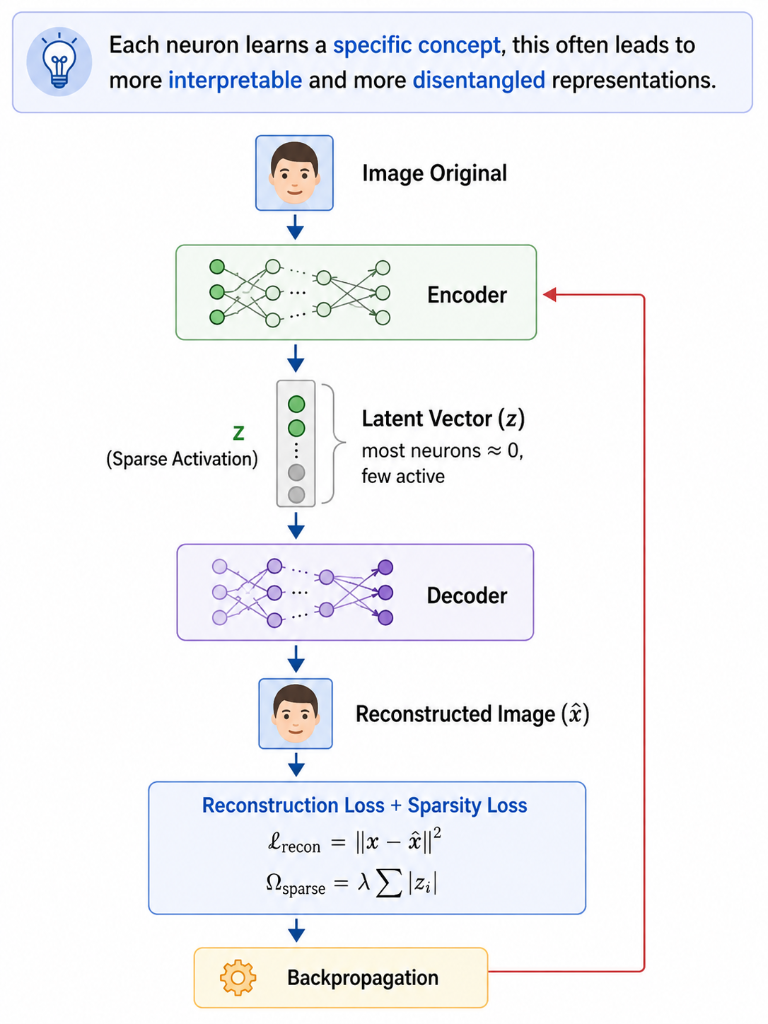
\includegraphics[width=0.85\linewidth]{figures/fig_8_sparse_autoencoder.png}
    \caption{Sparse Autoencoder architecture enforcing sparse latent activations where most neurons $\approx 0$ and only a few remain active.}
    \label{fig:sparse_autoencoder}
\end{figure}

\subsection{Objective Function \& Loss Formulation}
The reconstruction process is identical to a vanilla autoencoder; the primary difference lies in the loss function. Instead of minimizing only reconstruction error, we minimize the combined loss:
\[
\text{Total Loss} = \text{Reconstruction Loss} + \text{Sparsity Penalty}
\]
Formally, the total loss $\mathcal{L}_{\text{SAE}}$ combines standard reconstruction error with a sparsity penalty $\Omega_{\text{sparse}}(z)$:
\[
\mathcal{L}_{\text{SAE}} = \| x - \hat{x} \|^2 + \lambda \sum_i |z_i|
\]
The sparsity penalty discourages too many neurons from being active simultaneously. Common choices for the sparsity penalty include:
\begin{itemize}
    \item \textbf{$L_1$ Regularization}: Adds an $L_1$ norm penalty on latent activations $\sum_i |z_i|$.
    \item \textbf{KL Divergence}: Encourages a low average activation per neuron across training batches relative to a target sparsity parameter $\rho$.
\end{itemize}

\subsection*{Summary}
A Sparse Autoencoder has the same architecture as a vanilla autoencoder but adds a sparsity penalty to the loss function, encouraging only a small number of latent neurons to be active. This leads to compact, efficient, and highly interpretable feature representations.
